{\color{oorange}\subsection{Metodo del Gradiente Coniugato}}
Il metodo del gradiente coniugato è un algoritmo per la risoluzione di un sistema lineare la cui matrice associata  
è simmetrica e definita positiva,
 e consente di risolvere il sistema in un numero di iterazioni che è al massimo $n$ (in aritmetica esatta).

La funzione $f$ da minimizzare è data dalla formula
  $f(x) = \frac{1}{2} ||Ax - b||_2^2 $, il cui gradiente $\nabla f$ è dato da
$\nabla f(x) = A^TAx - A^Tb  $.

Utilizzando il metodo del gradiente coniugato implementato nella funzione \code{minimize}
 abbiamo calcolato la soluzione naive.

\begin{figure}[H]
  \centering
  \begin{subfigure}{0.9\textwidth}
    \centering
    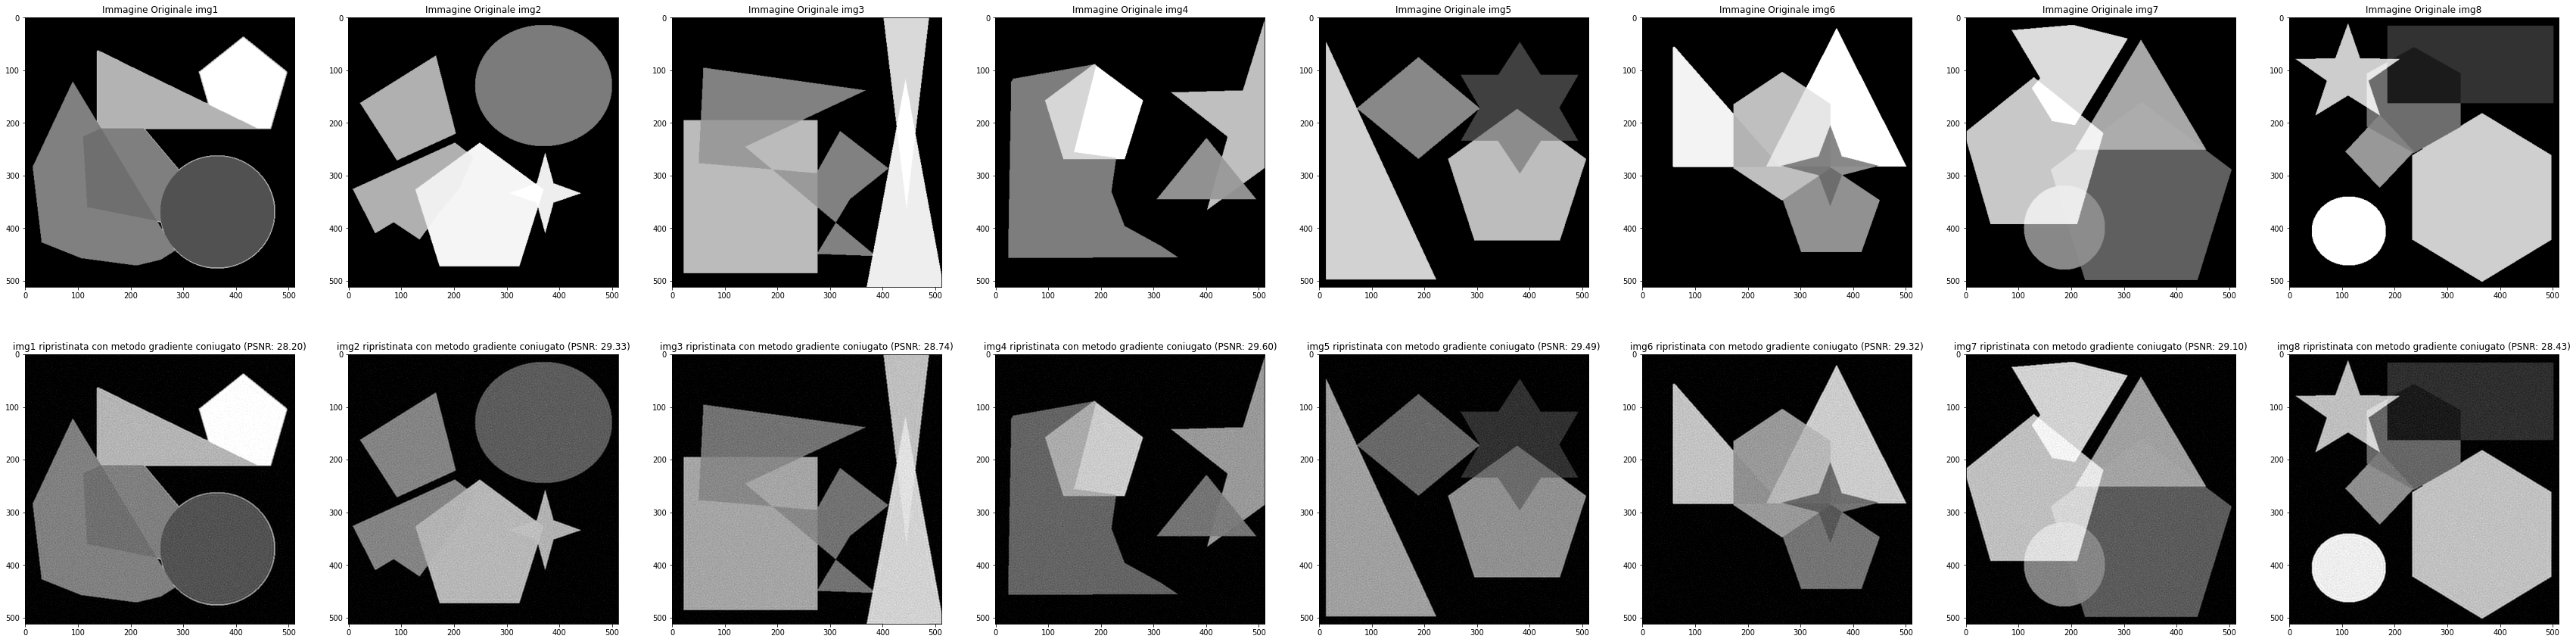
\includegraphics[width=0.9\textwidth]{imgRel/datasetconiugato.png}
    \caption{Immagini geometriche ripristinate con metodo del gradiente coniugato naive}
    \label{fig:geomripristinate}
  \end{subfigure}

  \begin{subfigure}{0.5\textwidth}
    \centering
    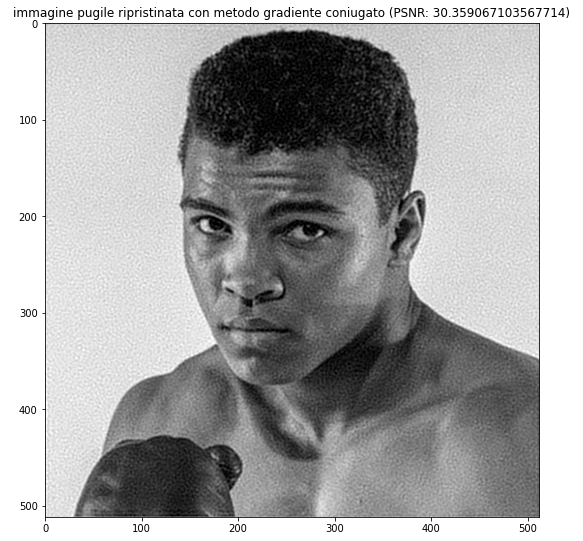
\includegraphics[width=0.6\textwidth]{imgRel/pugilemgc.png}
    \caption{Immagine ritratto ripristinata con metodo del gradiente coniugato naive}
    \label{fig:pugilemgc}
  \end{subfigure}\hfill
  \begin{subfigure}{0.5\textwidth}
    \centering
    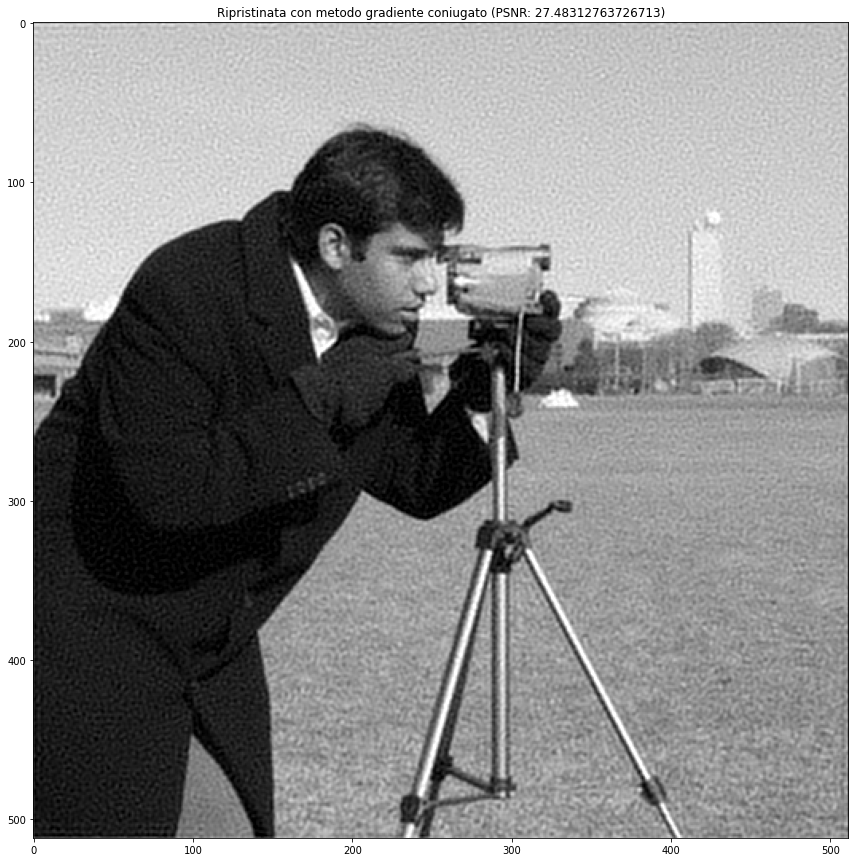
\includegraphics[width=0.6\textwidth]{MANCANTI/cameramanPuntoDueCG.png}
    \caption{Immagine con testo ripristinata con metodo del gradiente coniugato naive}
  \end{subfigure}
  \caption{Analisi immagini ripristinate con metodo del gradiente coniugato naive}
  \begin{minipage}{0.6\textwidth}\centering
    \begin{tabular}{|lcr|}
      \hline
      \rowcolor{orange}
      \multicolumn{1}{|c|}{\textbf{Immagine}} & \multicolumn{1}{l|}{\textbf{PSNR corrotte}} & \multicolumn{1}{c|}{\textbf{PSNR riprist.}}  \\ \hline
      img1.png          & 27.7886                      & 28.20                              \\
      img2.png          & 29.2539                      & 29.33                              \\
      img3.png          & 28.0014                      & 28.74                              \\
      img4.png          & 29.6382                      & 29.60                              \\
      img5.png          & 29.4566                      & 29.49                              \\
      img6.png          & 29.1727                      & 29.32                              \\
      img7.png          & 28.8132                      & 29.10                              \\
      img8.png          & 27.7142                      & 28.43                              \\ \hline
      pugile.png        & 30.3576                      & 30.36                              \\
      data.camera()     & 27.4138                      & 27.48                             \\ \hline
      \end{tabular}
      \captionof{table}{Valori PSNR delle immagini ricostruite con il metodo del gradiente coniugato naive}
  \end{minipage}
\end{figure}

\begin{figure}[H]
  \centering
    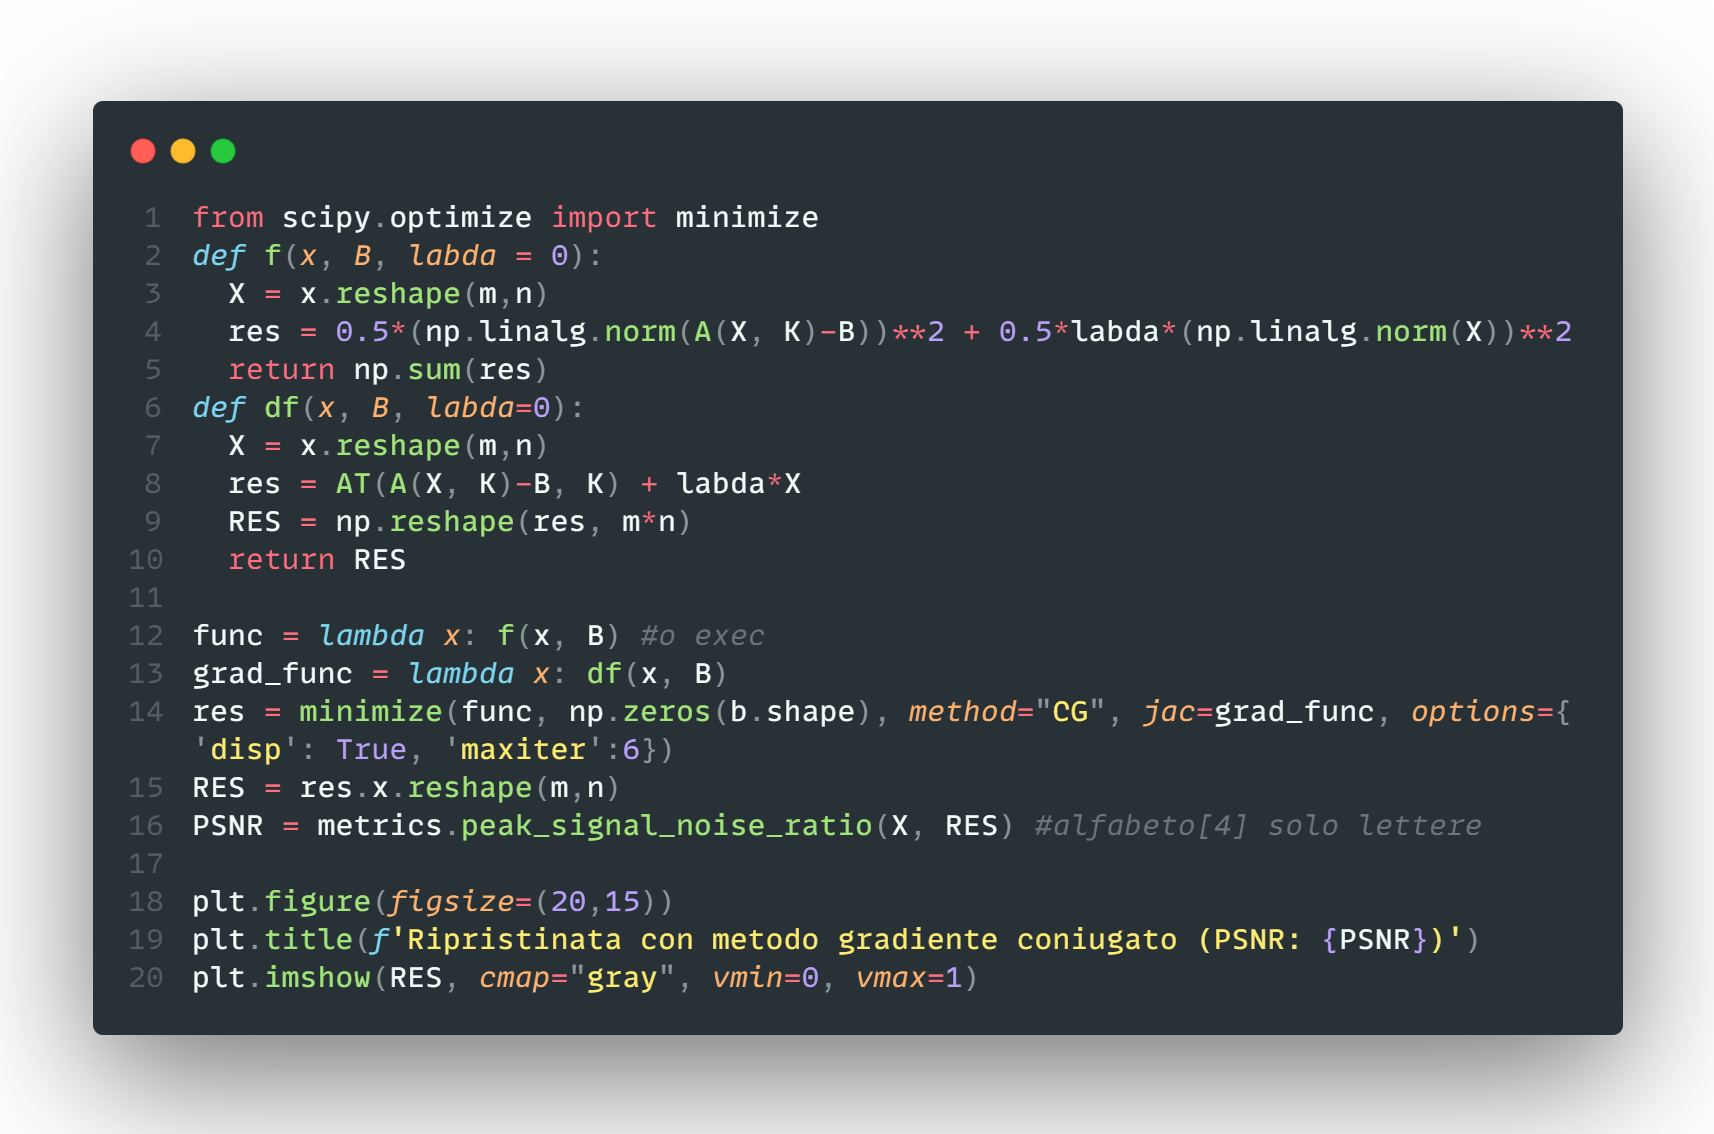
\includegraphics[width=0.6\textwidth]{imgCode/metGradCon.png}
    \caption{Codice in \code{Python 3} del Metodo del Gradiente Coniugato applicato ad una singola immagine}
    \label{fig:codeMGC}
\end{figure}

